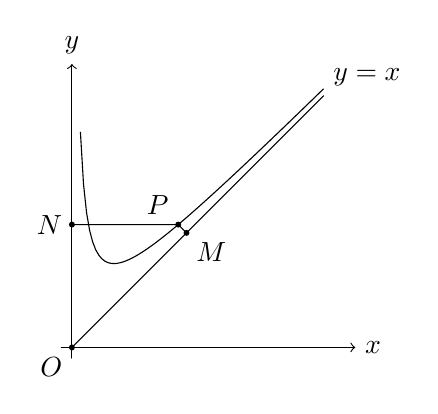
\begin{tikzpicture}[line cap=round,line join=round,scale=0.9]
  \coordinate (O) at (0,0);
  \coordinate (P) at (1.50,1.733333);
  \coordinate (N) at (0,1.733333);
  \coordinate (M) at (1.6166665,1.6166665);

  % Coordinate axes and the diagonal y=x.
  \draw[->] (0,-0.15)--(0,4.0) node[above] {$y$};
  \draw[->] (-0.15,0)--(4.0,0) node[right] {$x$};
  \draw (0,0)--(3.55,3.55) node[above right] {$y=x$};

  % Qualitative rescaling of x + c/x: positive and strictly convex for x>0.
  % The coefficient and coordinates are illustrative, not measurements from the source.
  \draw plot[domain=0.12:3.55,samples=80,variable=\x] ({\x},{\x+0.35/\x});

  % Projection from P to the y-axis and to y=x.
  \draw (P)--(N) (P)--(M);

  \fill (O) circle (1.2pt);
  \fill (P) circle (1.2pt);
  \fill (M) circle (1.2pt);
  \fill (N) circle (1.2pt);
  \node[below left] at (O) {$O$};
  \node[above left] at (P) {$P$};
  \node[left] at (N) {$N$};
  \node[below right] at (M) {$M$};
\end{tikzpicture}
